\chapter{Aplicaciones entre Espacios Topológicos}

\begin{definicion}
    Dados $(X, \cc{T})$, $(Y, \cc{T}')$ dos e.t., diremos que $f : (X, \cc{T}) \to (Y, \cc{T}')$ (que notaremos como $f:X \to Y$ cuando estén claros los e.t.) es \textbf{continua} en un punto $x_0\in X$ si $\forall N'\in \cc{N}_{f(x_0)}'$\ \ $\exists N \in \cc{N}_{x_0}$ con $f(N)\subset N'$. %TODO: dibujo

    \begin{center}
        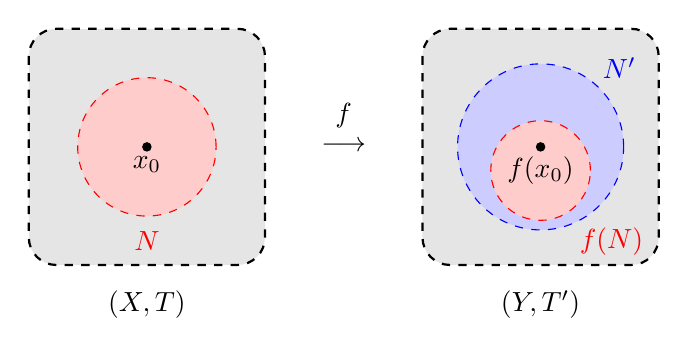
\begin{tikzpicture}
            \def\incolor{gray!20}

            \filldraw[rounded corners=10pt, dashed, thick, fill=\incolor] (0,0) rectangle (3,-3);

            \node at (1.5, -3.5) {$(X, \cc{T})$};
            \node at (4, -1.1) {$f$};
            \node at (4, -1.5) {$\longrightarrow$};

            \filldraw[rounded corners=10pt, dashed, thick, fill=\incolor] (5,0) rectangle (8,-3);

            \node at (6.5, -3.5) {$(Y, \cc{T}')$};

            \filldraw[dashed, draw=red, fill=red!20] (1.5, -1.5) circle (25pt);

            \node at (1.5, -2.7) {\textcolor{red}{$N$}};

            \filldraw[dashed, draw=blue, fill=blue!20] (6.5, -1.5) circle (30pt);

            \filldraw[dashed, draw=red, fill=red!20] (6.5, -1.8) circle (18pt);

            \node at (7.4, -2.7) {\textcolor{red}{$f(N)$}};

            \node at (7.5, -0.5) {\textcolor{blue}{$N'$}};

            \filldraw (1.5, -1.5) circle (1.5pt)  node[below] {$x_0$};

            \filldraw (6.5, -1.5) circle (1.5pt)  node[below] {$f(x_0)$};

            
        \end{tikzpicture}
    \end{center}

    Equivalentemente, $\forall N'\in \cc{N}_{f(x)}'$  $f^{-1}(N')\in \cc{N}_{x_0}$. Es decir, la imagen inversa por f de todo entorno de $f(x)$ en el espacio topológico $\cc{T}'$ es entorno de $x$ en el espacio topológico $\cc{T}$.
    \endsquare
\end{definicion}

\begin{observacion}
    La definición se puede reformular usando abiertos, abiertos básicos o entornos básicos. La demostración queda planteada como ejercicio para el lector. %TODO
    \endsquare
\end{observacion}

\begin{definicion}
    Dados $(X, \cc{T})$, $(Y, \cc{T}')$ dos e.t., $\emptyset \neq A\subset X$. Diremos que $f:X\to Y$ es \textbf{continua en $A$} si es continua en $x$\ \ $\forall x \in A$. Diremos que $f$ es \textbf{continua} si es continua en $X$.
    \endsquare
\end{definicion}

\begin{prop}
    Dados $(X, \cc{T})$, $(Y, \cc{T}')$ dos e.t., $f: X \to Y$. Entonces son equivalentes:
    \begin{enumerate}
        \item[(i)] $f$ es continua.
        \item[(ii)] $f^{-1}(U')\in \cc{T}$\ \ $\forall U' \in \cc{T}$ ($f$ trae abiertos en abiertos).
        \item[(iii)] $f^{-1}(B')\in \cc{T}$\ \ $\forall B'\in \cc{B}'$, donde $\cc{B}'$ es base de $\cc{T}'$.
        \item[(iv)] $f^{-1}(C')\in \cc{C}_{\cc{T}}$\ \ $\forall C' \in \cc{C}_{\cc{T}'}$ ($f$ trae cerrados en cerrados).
        \item[(v)] $f(\overline{A})\subset \overline{f(A)}$\ \ $\forall A \subset X$.
    \end{enumerate}

    \begin{proof}\
        \begin{enumerate}
            \item[(i)$\Rightarrow$(ii)] Supongamos que $f$ es continua. Tomamos $U' \in \cc{T}'$ y tendremos que verificar que $f^{-1}(U')\in \cc{T}$. Sea $x \in f^{-1}(U')$, entonces tendré que ver que $f^{-1}(U')\in \cc{N}_x$. Sabemos que $f(x)\in U' \subset \cc{N}_{f(x)}$. Como $f$ es continua, entonces $\exists U\in \cc{T} $, $x\in U$, $f(U)\subset U' \Rightarrow x \in U \subset f^{-1}(U')$. Como $U\in \cc{T}$, tenemos que $f^{-1}(U')\in \cc{N}_x$. Como esto sucede para un $x$ arbitrario tendremos que se verifica.
            \item[(ii)$\Rightarrow$(iii)] Esta implicación es trivial ya que todo abierto básico es en particular abierto en la topología.
            \item[(iii)$\Rightarrow$(iv)] Sea $C' \in \cc{C}_{\cc{T}'}$, $C'\subset Y$. Tendré que ver que $f^{-1}(C')\in \cc{C}_{\cc{T}}$, lo cual es equivalente a ver que $X \setminus f^{-1}(C')\in \cc{T}$. Sabemos que $X\setminus f^{-1}(C') = f^{-1}(Y\setminus C')$ y $Y\setminus C'\in \cc{T}$. Como $\cc{B}'$ es base de $\cc{T}'$, tenemos que $Y\setminus C'=\bigcup\limits_{i\in I} B_i'$ con $B_i'\in \cc{B}'$\ \ $\forall i \in I$. Entonces tenemos que $f^{-1}(Y\setminus C') = f^{-1}\left(\bigcup\limits_{i\in I}B_i'\right) = \bigcup\limits_{i\in I}f^{-1}(B_i')\in \cc{T}$ por ser unión de abiertos.
            \item[(iv)$\Rightarrow$(v)] Sea $\emptyset \neq A \subset X$, como $\overline{f(A)}\in \cc{C}_{\cc{T}'}$, por (iv) tenemos que $f^{-1}(\overline{f(A)})\in \cc{C}_{\cc{T}}$. Además, $A \subset f^{-1}(f(A))\subset f^{-1}(\overline{f(A)})\in \cc{C}_{\cc{T}}$. Entonces $\overline{A}\subset f^{-1}(\overline{f(A)})$. Al aplicar $f$ tenemos que $f(\overline{A})\subset f(f^{-1}(\overline{f(A)}))=\overline{f(A)}$.
            \item[(v)$\Rightarrow$(iv)] Sea $C' \in \cc{C}_{\cc{T}'}$ y tendremos que ver que $f^{-1}(C')\in \cc{C}_{\cc{T}}$. Para ello veré que coincide con su adherencia, es decir, que $\overline{f^{-1}(C')} = f^{-1}(C')$. Como la inclusión $\overline{f^{-1}(C')} \supset f^{-1}(C')$ es clara tendré que ver solo la otra incusión. Sea $A=f^{-1}(C')$, por (v) tenemos que $f(\overline{f^{-1}(C')})\subset \overline{f(f^{-1}(C'))} \subset \overline{C'}=C'$. Aplicando $f^{-1}$ tenemos que $f^{-1}(f(\overline{f^{-1}(C')}))\subset f^{-1}(C')$ y como $f^{-1}(f(\overline{f^{-1}(C')})) = \overline{f^{-1}(C')}$ tenemos lo buscado.
            \item[(iv)$\Rightarrow$(i)] Sea $x\in X$ arbitrario. Tendré que ver que $f$ es continua en $x$. Sea $U'\in \cc{T}'$ con $f(x)\in U'$. Tendré que ver que existe un $U\in \cc{T}$ con $x\in U$ y $f(U)\subset U'$. Tomo $Y\setminus(U')\in \cc{C}_{\cc{T}'}$ y por (iv) tenemos que $f^{-1}(Y\setminus U')\in \cc{C}_{\cc{T}}$ y $f^{-1}(Y\setminus U') = X \setminus f^{-1}(U')$ por lo que $x\in f^{-1}(U')\in \cc{T}$. Como $f(f^{-1}(U'))\subset U'$ puedo denotar $U = f^{-1}(U')$ y tenemos de nuevo lo buscado. 
        \end{enumerate}
    \end{proof}
\end{prop}

\begin{observacion}
    Si $f: (X, \cc{T}) \to (Y, \cc{T}')$ es una aplicación continua, entonces 
    \begin{gather*}
        f^{-1}((a,b)), f^{-1}((-\infty, b)), f^{-1}((a, +\infty))\in \cc{T}
    \end{gather*}
    y además 
    \begin{gather*}
        f^{-1}([a,b]), f^{-1}((-\infty, b]), f^{-1}([a, +\infty))\in \cc{C}_{\cc{T}}
    \end{gather*}
    La utilidad de esta observación es poder ver si un conjunto es abierto viendo si existe una aplicación continua que lleve un abierto de la topología en dicho conjunto. Análogamente se puede usar para cerrados.
    \endsquare
\end{observacion}

\begin{ejemplo}\
    \begin{itemize}
        \item $f:(X, d) \to (Y, d')$ continua entre espacios métricos 
        \begin{align*}
            \sii &\forall \veps >0\ \ \exists \delta >0 \text{ tal que si } d(x, x_0)<\delta \text{ entonces } d'(f(x), f(x_0))<\veps \sii\\
            \sii &\forall \veps >0 \ \ \exists \delta >0 \text{ tal que } f(B(x_0, \delta))\subset B'(f(x_0), \veps).
        \end{align*}
    \end{itemize}
\end{ejemplo}